\section{Verteilte Systeme}

\begin{definition}{Verteiltes System}\\
Ein Netzwerk aus autonomen Computern und Softwarekomponenten, die als einheitliches System erscheinen:
\begin{itemize}
    \item Autonome Knoten und Komponenten
    \item Netzwerkverbindung
    \item Erscheint dem Benutzer wie ein einzelnes, kohärentes System
\end{itemize}
\end{definition}

\begin{concept}{Charakteristika verteilter Systeme}\\
Typische Merkmale moderner verteilter Systeme:
\begin{itemize}
    \item \textbf{Skalierbarkeit:} Oft sehr große Systeme
    \item \textbf{Datenorientierung:} Zentrale Datenbanken
    \item \textbf{Interaktivität:} GUI und Batch-Verarbeitung
    \item \textbf{Nebenläufigkeit:} Parallele Benutzerinteraktionen
    \item \textbf{Konsistenz:} Hohe Anforderungen an Datenkonsistenz
\end{itemize}
\end{concept}

\begin{theorem}{Grundlegende Konzepte}\\
\textbf{1. Kommunikation:}
\begin{itemize}
    \item Remote Procedure Calls (RPC)
    \item Message Queuing
    \item Publish-Subscribe-Systeme
\end{itemize}

\textbf{2. Fehlertoleranz:}
\begin{itemize}
    \item Replikation von Komponenten
    \item Failover-Mechanismen
    \item Fehlererkennung und -behandlung
\end{itemize}

\textbf{3. Fehlersemantik:}
\begin{itemize}
    \item Konsistenzgarantien
    \item Recovery-Verfahren
    \item Kompensationsmechanismen
\end{itemize}
\end{theorem}


\begin{concept}{Kommunikationsmodelle}\\
\textbf{1. Synchrone Kommunikation}
\begin{itemize}
    \item Synchroner entfernter Dienstaufruf $\rightarrow$ blockierend
    \item Sender wartet auf Ergebnis der Methode send
    \item Typisch für Request-Response Pattern
\end{itemize}

\textbf{2. Asynchrone Kommunikation}
\begin{itemize}
    \item Asynchroner entfernter Serviceaufruf $\rightarrow$ nicht blockierend
    \item Sender kann direkt weitermachen
    \item Senden und Empfangen zeitlich versetzt
    \item Keine Blockierung des Prozesses
\end{itemize}
\end{concept}


\begin{example2}{Prüfungsaufgabe: Kommunikationsanalyse}\\
\textbf{Szenario:}
Ein verteiltes System soll große Datenmengen verarbeiten. Analysieren Sie die Vor- und Nachteile synchroner vs. asynchroner Kommunikation.

\begin{minipage}[t]{0.5\textwidth}
    \textbf{Synchrone Kommunikation:}
    \begin{itemize}
        \item \textbf{Vorteile:}
        \begin{itemize}
            \item Einfaches \\Programmiermodell
            \item Direktes Feedback
            \item Garantierte Reihenfolge
        \end{itemize}
        \item \textbf{Nachteile:}
        \begin{itemize}
            \item Blockierung von Ressourcen
            \item Schlechte Skalierbarkeit
            \item Anfällig für Timeouts
        \end{itemize}
    \end{itemize}
\end{minipage}
\begin{minipage}[t]{0.5\textwidth}
    \textbf{Asynchrone Kommunikation:}
    \begin{itemize}
        \item \textbf{Vorteile:}
        \begin{itemize}
            \item Bessere Ressourcennutzung
            \item Höhere Skalierbarkeit
            \item Entkopplung von Systemen
        \end{itemize}
        \item \textbf{Nachteile:}
        \begin{itemize}
            \item Komplexere Implementierung
            \item Schwierigere\\ Fehlerbehandlung
            \item Reihenfolge nicht garantiert
        \end{itemize}
    \end{itemize}
\end{minipage}
\end{example2}

\begin{theorem}{Kommunikation zwischen Client und Server}\\
\textbf{Grundlagen:}
\begin{itemize}
    \item Services sind über URLs aufrufbar: \\protokoll://<server>:<port>/<pfad\_des\_service>
    \item Kommunikation über TCP oder UDP
    \item Socket = Programmierschnittstelle zu Kommunikationskanal
    \item IP-Socket-Adresse besteht aus IP-Adresse + Portnummer
\end{itemize}

\textbf{Ablauf:} study THIN :)
\end{theorem}

\begin{corollary}{Lebenszyklus von Serverbausteinen}\\
Ein Serverbaustein durchläuft verschiedene Zustände:
\begin{itemize}
    \item Wird zur Laufzeit von Server instanziiert
    \item Zustandsübergänge abhängig von Bausteintyp und Implementierung
    \item Anzahl und Benennung der Zustände variiert je nach Middleware
\end{itemize}
\end{corollary}

\begin{corollary}{Heterogenität}\\
Mehrere Ebenen der Heterogenität müssen berücksichtigt werden:

\textbf{1. Hardware und Betriebssysteme}
\begin{itemize}
    \item Unterschiedliche Speicherung der Daten\\ ("Little Endian" vs "Big Endian")
    \item Verschiedene Zeichensätze (ASCII, EBCDIC, Unicode)
\end{itemize}

\textbf{2. Überwindung der Heterogenität}
\begin{itemize}
    \item Einheitliche Transportsyntax (ASN.1, XDR, HTML, XML, JSON)
    \item Middleware-Technologien mit standardisierten Ansätzen
    \item Marshalling/Unmarshalling über generierten Code
\end{itemize}
\end{corollary}

\begin{definition}{Middleware} ist eine Softwareschicht, die standardisierte Kommunikations- und andere Dienste über ein API bereitstellt.

\textbf{Middleware-Kategorien:}
\begin{itemize}
    \item \textbf{Anwendungsorientiert:}
    \begin{itemize}
        \item Java Enterprise Edition (Jakarta EE)
        \item Spring-Framework
        \item .NET Enterprise Services
    \end{itemize}
    
    \item \textbf{Kommunikationsorientiert:}
    \begin{itemize}
        \item Remote Procedure Call (RPC)
        \item Remote Method Invocation (RMI)
        \item CORBA (Common Object Request Broker Architecture)
        \item REST, WebSocket
        \item RESTful APIs, GraphQL
    \end{itemize}
    
    \item \textbf{Nachrichtenorientiert:}
    \begin{itemize}
        \item Message Oriented Middleware (MOM)
        \item Java Messaging Service (JMS)
        \item Message Broker (MQTT, RabbitMQ, Kafka)
    \end{itemize}
\end{itemize}
\end{definition}

\begin{concept}{Marshalling/Unmarshalling}\\
Umwandlung von Daten für die Übermittlung:

\textbf{1. Tag-basierte Transfersyntax}
\begin{itemize}
    \item ASN.1 mit BER (Basic Encoding Rules)
    \item TLV-Kodierung (Type, Length, Value)
\end{itemize}

\textbf{2. Tag-freie Transfersyntax}
\begin{itemize}
    \item Sun ONC XDR, CORBA CDR
    \item Beschreibung durch Stellung in Nachricht
    \item Aufbau beiden Seiten bekannt
\end{itemize}

\textbf{3. Moderne Formate}
\begin{itemize}
    \item XML (Tag-basiert)
    \item JSON (Tag-basiert, sprachunabhängig)
\end{itemize}
\end{concept}








\begin{KR}{Entwurf verteilter Systeme}
\paragraph{1. Systemanalyse}
\begin{itemize}
    \item Anforderungen identifizieren
    \item Verteilungsaspekte analysieren
    \item Konsistenzanforderungen definieren
\end{itemize}

    \begin{minipage}[t]{0.5\textwidth}
        \begin{itemize}
            \item \textbf{Funktional:}
        \begin{itemize}
            \item Kernfunktionalitäten
            \item Datenmodell
            \item Schnittstellen
        \end{itemize}
    \end{itemize}
    \end{minipage}
    \begin{minipage}[t]{0.5\textwidth}
        \begin{itemize}
            \item \textbf{Nicht-funktional:}
        \begin{itemize}
            \item Skalierbarkeit
            \item Verfügbarkeit
            \item Latenz
        \end{itemize}
    \end{itemize}
    \end{minipage}

\paragraph{2. Architekturentscheidungen}
\begin{itemize}
    \item Architekturstil wählen
    \item Kommunikationsmuster festlegen
    \item Fehlertoleranzstrategie definieren
\end{itemize}

    \begin{minipage}[t]{0.5\textwidth}
        \begin{itemize}
            \item \textbf{Kommunikation:}
        \begin{itemize}
            \item Synchron vs. Asynchron
            \item Push vs. Pull
            \item Protokollwahl
        \end{itemize}
    \end{itemize}
    \end{minipage}
    \begin{minipage}[t]{0.5\textwidth}
        \begin{itemize}
            \item \textbf{Datenmanagement:}
        \begin{itemize}
            \item Sharding
            \item Replikation
            \item Caching
        \end{itemize}
    \end{itemize}
    \end{minipage}
    
\paragraph{3. Technologieauswahl/Implementierungsaspekte}
\begin{itemize}
    \item Middleware evaluieren
    \item Protokolle bestimmen
    \item Werkzeuge auswählen
\end{itemize}

    \begin{minipage}[t]{0.5\textwidth}
        \begin{itemize}
            \item \textbf{Middleware:}
        \begin{itemize}
            \item REST
            \item gRPC
            \item Apache Kafka
        \end{itemize}
    \end{itemize}
    \end{minipage}
    \begin{minipage}[t]{0.5\textwidth}
        \begin{itemize}
            \item \textbf{Implementierung:}
        \begin{itemize}
            \item Nebenläufigkeit
            \item Fehlersituationen
            \item Parameterübergabe
        \end{itemize}
    \end{itemize}
    \end{minipage}
\end{KR}


\subsubsection{Architekturmodelle / Architekturstile}

\begin{definition}{Architekturmodelle}\\
Heute finden vor allem folgende Architekturmodelle ihren Einsatz:

\textbf{1. Client/Server}
\begin{itemize}
    \item Kurzlebiger Client-Prozess kommuniziert mit langlebigem Server-Prozess
    \item Beispiel: Web-Applikation
\end{itemize}

\textbf{2. Peer-to-Peer}
\begin{itemize}
    \item Gleichberechtigte Peer-Prozesse
    \item Informationsaustausch nur bei Bedarf
    \item Beispiel: Blockchain
\end{itemize}

\textbf{3. Event Systems} (Publish-Subscribe)
\begin{itemize}
    \item Event-Sources-Prozesse und Event-Sinks-Prozesse
    \item Asynchroner Informationsaustausch
    \item Beispiel: E-Mail-System
\end{itemize}
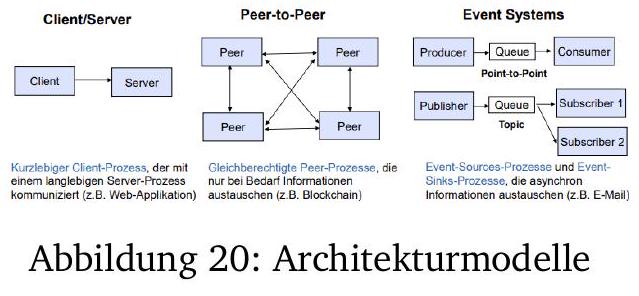
\includegraphics[width=0.9\linewidth]{images/2024_12_29_0d1d7b5551ea1b4b41bdg-18}
\end{definition}



\begin{KR}{Verteilungsprobleme analysieren}

    \begin{minipage}[t]{0.5\textwidth}
        \textbf{1. Probleme identifizieren}
        \begin{itemize}
            \item \textbf{Netzwerk:}
            \begin{itemize}
                \item Latenz
                \item Bandbreite
                \item Ausfälle
            \end{itemize}
            \item \textbf{Daten:}
            \begin{itemize}
                \item Konsistenz
                \item Replikation
                \item Synchronisation
            \end{itemize}
            \item \textbf{System:}
            \begin{itemize}
                \item Skalierung
                \item Verfügbarkeit
                \item Wartbarkeit
            \end{itemize}
        \end{itemize}
    \end{minipage}
    \begin{minipage}[t]{0.5\textwidth}
        \textbf{2. Lösungsstrategien entwickeln}
        \begin{itemize}
            \item \textbf{Netzwerk:}
            \begin{itemize}
                \item Caching
                \item Compression
                \item Redundanz
            \end{itemize}
            \item \textbf{Daten:}
            \begin{itemize}
                \item Eventual Consistency
                \item Master-Slave Replikation
                \item Konfliktauflösung
            \end{itemize}
            \item \textbf{System:}
            \begin{itemize}
                \item Load Balancing
                \item Service Discovery
                \item Circuit Breaker
            \end{itemize}
        \end{itemize}
    \end{minipage}
\end{KR}



\begin{example2}{Prüfungsaufgabe: Systemanalyse}
\textbf{Aufgabe:}
Für ein Online-Banking-System sollen kritische Aspekte analysiert werden.

\textbf{1. Anforderungen identifizieren:}
\begin{itemize}
    \item Hohe Verfügbarkeit (24/7)
    \item Strikte Konsistenz bei Finanztransaktionen
    \item Skalierbarkeit für viele Nutzer
    \item Sicherheit und Verschlüsselung
\end{itemize}

\textbf{2. Architekturentscheidungen:}
\begin{itemize}
    \item \textbf{Client-Server mit Multi-Tier:}
    \begin{itemize}
        \item Präsentationsschicht (Web/Mobile)
        \item Geschäftslogik
        \item Datenbankschicht
    \end{itemize}
    
    \item \textbf{Synchrone Kommunikation:}
    \begin{itemize}
        \item Direkte Bestätigung von Transaktionen
        \item Garantierte Reihenfolge
    \end{itemize}
\end{itemize}

\textbf{3. Technische Maßnahmen:}
\begin{itemize}
    \item Verteilte Datenbank mit Two-Phase Commit
    \item Load Balancing für Hochverfügbarkeit
    \item SSL/TLS für Verschlüsselung
    \item Session Management für Authentifizierung
\end{itemize}
\end{example2}

\begin{example2}{Typische Prüfungsaufgabe: CAP-Theorem}\\
\textbf{Aufgabe:}
Analysieren Sie für ein verteiltes Datenbanksystem die Auswirkungen des CAP-Theorems.

\textbf{CAP-Theorem Komponenten:}
\begin{itemize}
    \item \textbf{Consistency:} Alle Knoten sehen dieselben Daten
    \item \textbf{Availability:} Jede Anfrage erhält eine Antwort
    \item \textbf{Partition Tolerance:} System funktioniert trotz Netzwerkausfällen
\end{itemize}

\textbf{Analyse der Trade-offs:}
\begin{itemize}
    \item \textbf{CA-System:}
    \begin{itemize}
        \item Hohe Konsistenz und Verfügbarkeit
        \item Keine Netzwerkpartitionierung möglich
        \item Beispiel: Traditionelle RDBMS
    \end{itemize}
    \item \textbf{CP-System:}
    \begin{itemize}
        \item Konsistenz und Partitionstoleranz
        \item Eingeschränkte Verfügbarkeit
        \item Beispiel: MongoDB
    \end{itemize}
    \item \textbf{AP-System:}
    \begin{itemize}
        \item Verfügbarkeit und Partitionstoleranz
        \item Eventual Consistency
        \item Beispiel: Cassandra
    \end{itemize}
\end{itemize}
\end{example2}


\begin{KR}{Design Pattern Auswahl}\\
    %todo actually put the patterns we talked about in the lecture here
\textbf{1. Remote Proxy Pattern}
\begin{itemize}
    \item Grundlegendes Pattern für Zugriff auf Services
    \item Proxy wird durch Dependency Injection (DI) instanziiert
    \item Client- und serverseitiger Stub ("Skeleton")
\end{itemize}

\textbf{2. Data Transfer Object (DTO)}
\begin{itemize}
    \item Bündelt mehrere Daten für einen einzelnen Programmaufruf
    \item Reduziert Anzahl der Remote-Zugriffe
    \item Typischerweise "immutable" (nur getter-Methoden)
\end{itemize}

\textbf{3. Service Locator}
\begin{itemize}
    \item Zentrale Registrierung von Services
    \item Ermöglicht dynamisches Auffinden von Diensten
    \item Unterstützt Load Balancing
\end{itemize}
\end{KR}

\begin{example2}{Prüfungsaufgabe: Architekturmuster-Analyse}\\
\textbf{Szenario:}
Ein Messaging-System soll entwickelt werden, das folgende Anforderungen erfüllt:
\begin{itemize}
    \item Hohe Skalierbarkeit
    \item Keine zentrale Komponente (Single Point of Failure)
    \item Direkter Nachrichtenaustausch zwischen Nutzern
    \item Offline-Fähigkeit
\end{itemize}

\textbf{Analysieren Sie die Architekturmuster:}

\textbf{1. Client-Server}
\begin{itemize}
    \item \textbf{Vorteile:}
    \begin{itemize}
        \item Zentrale Verwaltung
        \item Einfache Konsistenzsicherung
    \end{itemize}
    \item \textbf{Nachteile:}
    \begin{itemize}
        \item Single Point of Failure
        \item Skalierungsprobleme
    \end{itemize}
\end{itemize}

\textbf{2. Peer-to-Peer}
\begin{itemize}
    \item \textbf{Vorteile:}
    \begin{itemize}
        \item Keine zentrale Komponente
        \item Direkte Kommunikation
        \item Gute Skalierbarkeit
    \end{itemize}
    \item \textbf{Nachteile:}
    \begin{itemize}
        \item Komplexe Konsistenzsicherung
        \item Schwierige Verwaltung
    \end{itemize}
\end{itemize}

\textbf{Empfehlung:} Peer-to-Peer mit hybriden Elementen
\end{example2}

\begin{KR}{Typische Fehlerquellen}\\
\textbf{1. Netzwerkfehler}
\begin{itemize}
    \item Verbindungsabbrüche
    \item Timeouts
    \item Partitionierung
\end{itemize}

\textbf{2. Konsistenzprobleme}
\begin{itemize}
    \item Race Conditions
    \item Veraltete Daten
    \item Lost Updates
\end{itemize}

\textbf{3. Skalierungsprobleme}
\begin{itemize}
    \item Lastverteilung
    \item Resource-Management
    \item Bottlenecks
\end{itemize}

\textbf{Lösungsstrategien:}
\begin{itemize}
    \item Circuit Breaker Pattern
    \item Retry mit Exponential Backoff
    \item Idempotente Operationen
    \item Optimistic Locking
\end{itemize}
\end{KR}


\columnbreak


\begin{KR}{Implementierung verteilter Systeme}\\
\textbf{1. Nebenläufigkeit}
\begin{itemize}
    \item Iterative oder parallele Serverbausteine
    \item Threadpooling für gleichzeitige Bedienung mehrerer Clients
    \item Dispatcher verteilt Requests auf Threads
    \item Einfaches sequentielles Programmiermodell für Entwickler
\end{itemize}

\textbf{2. Fehlersituationen}
\begin{itemize}
    \item Request geht verloren
    \item Server-Response geht verloren
    \item Server stürzt während Ausführung ab
    \item Server braucht zu lange für Bearbeitung
    \item Client stürzt vor Ankunft des Ergebnisses ab
\end{itemize}

\textbf{3. Parameterübergabe}
\begin{itemize}
    \item Call-by-value: Wert wird übergeben
    \item Call-by-reference: Verweis auf Variable wird übergeben  
    \item Call-by-copy/restore: Aufrufer arbeitet mit Kopie
\end{itemize}
\end{KR}





\begin{example2}{Implementierungsaspekte}
\textbf{Zustandsverwaltung:}
\begin{itemize}
    \item \textbf{Stateful vs. Stateless:}
    \begin{itemize}
        \item Stateless Server bevorzugt
        \item Zustand in Datenbank oder Client
        \item Bessere Skalierbarkeit
    \end{itemize}
    
    \item \textbf{Session Management:}
    \begin{itemize}
        \item Verteilte Sessions
        \item Session Clustering
        \item Sticky Sessions
    \end{itemize}
\end{itemize}

\textbf{Garbage Collection:}
\begin{itemize}
    \item Verteiltes Reference-Counting
    \item Leases für temporäre Ressourcen
    \item Zusammenarbeit mit lokalem GC
\end{itemize}
\end{example2}

\begin{KR}{Lastverteilung und Skalierung}\\
\textbf{1. Load Balancing}
\begin{itemize}
    \item Lastverteiler für multiple Serverinstanzen
    \item DNS-basiertes Request-Routing
    \item Session-Sticky Load Balancing
\end{itemize}

\textbf{2. Hochverfügbarkeit}
\begin{itemize}
    \item Server-Cluster
    \item Failover-Mechanismen
    \item Session-Replikation
\end{itemize}

\textbf{3. Skalierungsmethoden}
\begin{itemize}
    \item \textbf{Horizontal:} Mehr Rechner hinzufügen
    \item \textbf{Vertikal:} Ressourcen pro Rechner erhöhen
    \item \textbf{Funktional:} Services aufteilen
\end{itemize}
\end{KR}






